\documentclass[a4paper,12pt]{article}
\usepackage[utf8]{inputenc}
\usepackage{hyperref}
\usepackage{geometry}
\usepackage{titlesec}
\usepackage{graphicx} % Required for including images
\usepackage{enumitem}
\usepackage{lmodern}
\usepackage{titling}
\usepackage{xcolor}
\usepackage{placeins}

\geometry{margin=1in}
\titleformat{\section}{\normalfont\Large\bfseries}{\thesection.}{1em}{}
\title{Final Technical Report: Contributions and Justifications}
\author{Félicien Moquet}
\date{\vspace{-1.5em}}

\begin{document}

\maketitle
\tableofcontents
\newpage

\section{Introduction}
In this project, my contributions focused on delivering robust, usable, and legally responsible features. These efforts included the integration of documentation services, real-time email functionality, client-side validation mechanisms, and streamlined public deployment.

The aim was to ensure both technical operability and a clear user experience while respecting the legal obligations of AI monitoring tools.

\section{User Documentation Service}
A comprehensive user manual was created and made available in PDF format. This documentation provides first-time users with detailed instructions, complete with screenshots, explaining how to navigate the AI-powered proctoring system.

It includes:
\begin{itemize}
    \item Webcam activation
    \item Email registration
    \item Session result interpretation
    \item Common troubleshooting tips
\end{itemize}

\noindent\textbf{Link:} \href{https://fefe29.github.io/Automated-Online-Test-Monitoring-System_V4/user_doc.pdf}{User Documentation PDF}

\section{Privacy Policy Integration}
A privacy policy was developed to clarify the system’s scope and ethical use. It outlines how data is (or isn’t) stored, the probabilistic nature of AI, and warns that results should not be used for punitive actions without human oversight.

Users must explicitly accept this policy via a checkbox before beginning any session. This ensures GDPR-style compliance and informed consent.

\noindent\textbf{Link:} \href{https://fefe29.github.io/Automated-Online-Test-Monitoring-System_V4/privacy_policy.pdf}{Privacy Policy PDF}

\section{Email Sending Service: Design \& Robustness}
A real-time notification feature was implemented using \texttt{EmailJS}, a client-side email dispatching API. It enables the system to send session summaries to both candidate and sponsor immediately after the monitoring session ends.

\subsection*{Justification for EmailJS}
\begin{itemize}
    \item \textbf{No backend required:} It runs fully in-browser, avoiding the need for Node.js, server APIs, or SMTP configuration.
    \item \textbf{Quick integration:} EmailJS has native JavaScript support, which fit well with our Vite/React stack.
    \item \textbf{Asynchronous}: The API uses Promises, which simplifies error handling and feedback via \texttt{async/await}.
\end{itemize}

\subsection*{Limitations}
\begin{itemize}
    \item The free tier limits to 200 emails/month.
    \item Email addresses can be spoofed unless tied to a verified sender.
    \item EmailJS does not guarantee GDPR or HIPAA compliance.
\end{itemize}

\subsection*{Error Handling \& Validation}
The \texttt{sendEmail()} function was written to include:
\begin{itemize}
    \item \textbf{Strict input validation:} All three fields (results, candidate email, sponsor email) are checked.
    \item \textbf{Regex-based email format validation}.
    \item \textbf{Error propagation:} Wrapped in \texttt{try/catch} to prevent UI crash and log detailed feedback.
    \item \textbf{Alerts:} Visual feedback is immediately provided to users via small red error messages or alerts.
\end{itemize}

\section{Client-Side Validation and UX}
To ensure the user enters valid and complete information, multiple layers of validation were added in the \texttt{ButtonHandler.jsx} component:
\begin{itemize}
    \item Required fields: Empty inputs are blocked with an error message.
    \item Real-time checkbox monitoring: The "Terms of Use" box must be checked.
    \item Conditional rendering: Errors only appear after attempting to start the session, keeping the form clean.
    \item \textbf{Visual feedback:} Invalid or missing input displays red error messages in smaller font, styled with CSS.
\end{itemize}

\subsection*{Error Visibility Logic}
Errors are only displayed once the user clicks "Start Session". This avoids overwhelming the user on initial load, while still enforcing strict validation.


\section{Diagrams}
To better illustrate the system's architecture and workflow on the user interface, I created the following diagrams:

\begin{figure}[h!]
    \centering
    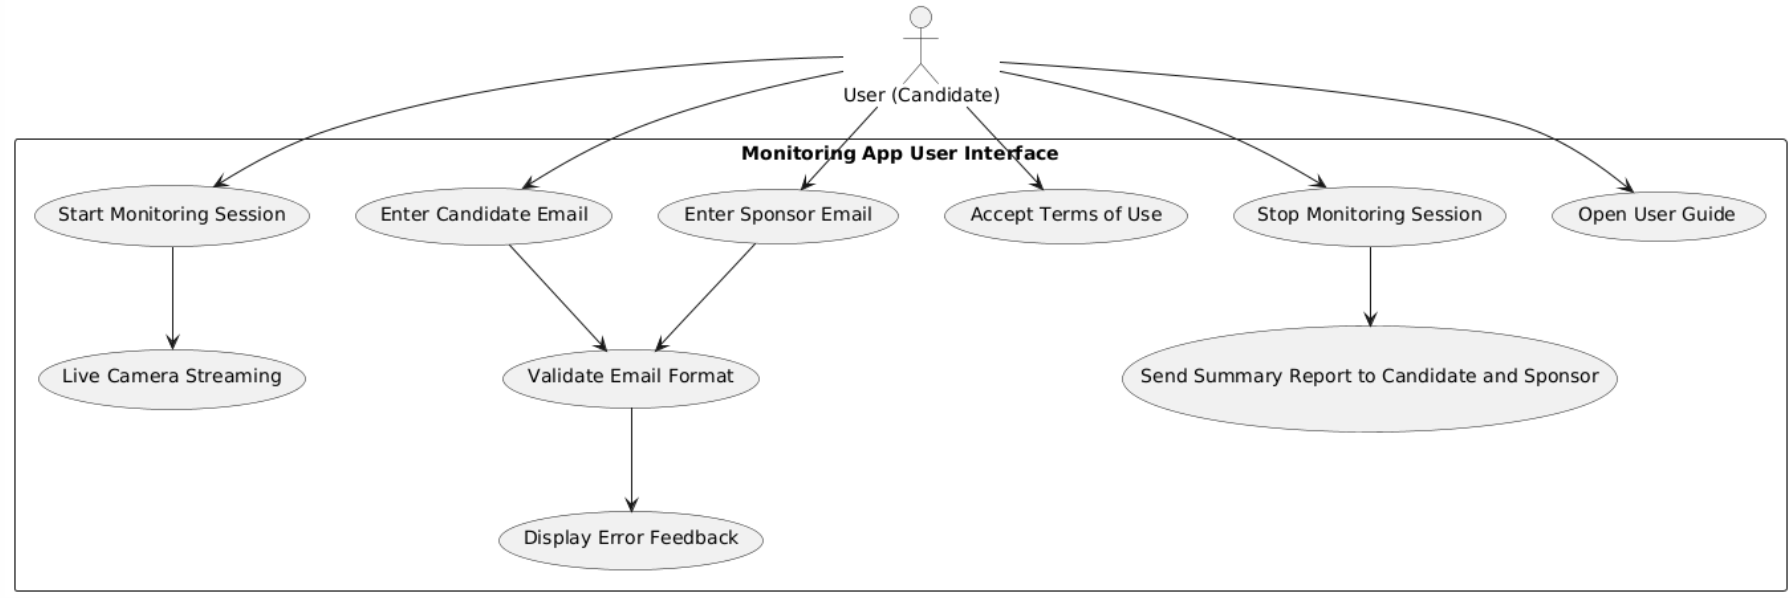
\includegraphics[width=0.8\textwidth]{IMG/use_case.png}
    \caption{User interface use case diagram}
    \label{fig:Use case diagram}
\end{figure}
\FloatBarrier

\begin{figure}[h!]
    \centering
    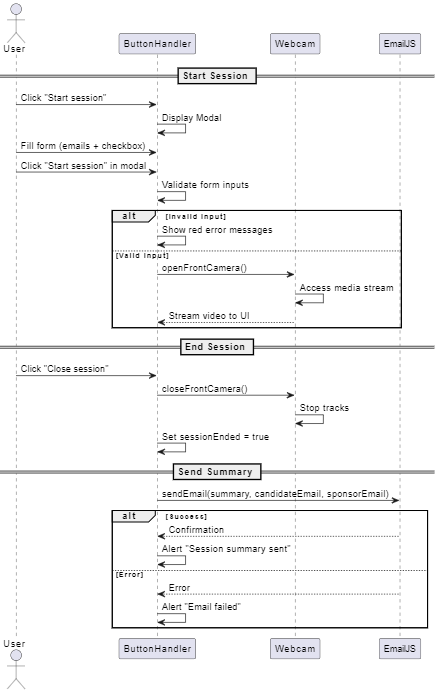
\includegraphics[width=0.5\textwidth]{IMG/sequentiel.png}
    \caption{User Interface Workflow Diagram: This diagram illustrates the user flow, from starting a session to receiving email summaries.}
    \label{fig:workflow_diagram}
\end{figure}
\FloatBarrier

\section{First Deployment Strategy: GitHub Pages}

Initially, the project was deployed publicly using GitHub Pages (as we had only a frontend app at this time), leveraging the \texttt{/docs} directory in the repository. This offered a lightweight, quick way to demo the application and validate user-facing functionality without infrastructure costs.\\

Additionally, since the project was already hosted and version-controlled on GitHub, using GitHub Pages significantly simplified deployment during the testing phase. It required no external setup, allowing us to iterate rapidly and publish updates directly from the development branch.


% \subsection*{Why GitHub Pages?}
% \begin{itemize}
%     \item \textbf{Lightweight:} No backend or server infrastructure was needed.
%     \item \textbf{Fast setup:} GitHub Pages is ideal for static frontend apps.
%     \item \textbf{Free and version-controlled:} Git integration makes deployments traceable.
% \end{itemize}

\subsection*{Deployment Process}
\begin{itemize}
    \item \texttt{vite.config.js} was configured to set \texttt{base: "./"} and output the build to \texttt{docs/}.
    \item PDF files such as the user manual and privacy policy were manually copied post-build.
    \item A custom \texttt{yarn deploy} script automates the build, commit, and push process.
\end{itemize}

\subsection*{Problems Encountered}
\begin{itemize}
    \item \textbf{PDF overwrite issues:} The Vite build occasionally deleted non-code assets unless copied after the build step.
    \item \textbf{Invisible file changes:} Git would not detect modified binaries like PDFs unless explicitly forced.
    \item \textbf{CI/CD errors:} GitHub Actions failed due to phantom submodule links in \texttt{node\_modules/.cache}.
\end{itemize}

\subsection*{Migration to AWS by Kateryna}
After validating the GitHub Pages deployment, \textbf{Kateryna redeployed the system with a full backend on AWS Cloud infrastructure}.

The initial GitHub Pages version was kept as a test/demo environment, while the AWS deployment serves as the foundation for a more robust production-ready architecture.

\section{Possible Improvements}
\begin{itemize}
    \item \textbf{Custom domain:} To remove GitHub branding and offer a clean URL.
    \item \textbf{Server-based email service:} Replace EmailJS with a backend like NodeMailer + Gmail API or SendGrid.
    \item \textbf{Dedicated email address:} Create a system-specific email address for sending notifications, as the current implementation uses my personal email with EmailJS (on github Pages) or Kateryna's one (on AWS).
    \item \textbf{Security:} Add CSP headers, reCAPTCHA, and token-based user validation.
    \item \textbf{AI Improvements:} Current spoof detection model could be improved with post-processing or ensemble models.
    \item \textbf{Monitoring dashboard:} Add an admin UI to track sessions, logs, and detection stats (now allowed thanks to AWS and the backend system).
\end{itemize}

\section{Personal Evaluation}
This project allowed me to develop skills at the crossroads of UX design, frontend engineering, ethical AI deployment, and devops automation.

My focus was on making the system:
\begin{itemize}
    \item Intuitive to use (via clear UI and documentation)
    \item Legally responsible (via policy agreements)
    \item Technically robust (with validation, exception handling, and fallback alerts)
\end{itemize}


\end{document}
